%%%%%%%%%%%%%%%%%%%%%%%%%%%%%%%%%%%%%%%%%%%%%%%%%%%%%%%%%%%%%%%
%
% Welcome to Overleaf --- just edit your article on the left,
% and we'll compile it for you on the right. If you give 
% someone the link to this page, they can edit at the same
% time. See the help menu above for more info. Enjoy!
%
%%%%%%%%%%%%%%%%%%%%%%%%%%%%%%%%%%%%%%%%%%%%%%%%%%%%%%%%%%%%%%%
%
% For more detailed article preparation guidelines, please see:
% http://f1000research.com/author-guidelines

\documentclass[10pt,a4paper,twocolumn]{article}
\usepackage{f1000_styles}
\usepackage{multirow} 
%% Default: numerical citations
\usepackage[numbers]{natbib}

%% Uncomment this lines for superscript citations instead
% \usepackage[super]{natbib}

%% Uncomment these lines for author-year citations instead
% \usepackage[round]{natbib}
% \let\cite\citep

\begin{document}

\title{\textit{F1000Research} Evaluating Metagenome Assembly on a Complex Community}
\titlenote{ }
\author[1]{Sherine Awad}
\author[2]{Luiz Irber}
\author[3]{C. Titus Brown}
\affil[1,2,3]{Department of Population Health and Reproduction, University of California, Davis, California}
 

\maketitle
\thispagestyle{fancy}

% Please list all authors that played a significant role in the research involved in the article. Please provide full affiliation information (including full institutional address, ZIP code and e-mail address) for all authors, and identify who is/are the corresponding author(s).

\begin{abstract}
 

 
Metagenome assembly is a challenging problem due to the biodiversity
of the microorganisms. Most assemblers are designed for whole genome
assembly and not capable of dealing with metagenomic samples. However,
in order to decide which assembler works best for metagenome, we need
to evaluate metagenome assembly generated by each assembler.

% CTB: mention microdiversity, species foo.

In this paper, we used three assemblers ; IDBA-UD, SPAdes, and Megahit
to assemble metagenome mock community data and evaluate the assembly
process in terms of resources utilization, assembly quality, genome
fraction covered, duplication ratio, misassemblies and partial
alignments.

The results show only small differences in content recovery between
assemblers. However, Megahit is much faster and produces shorter
contig lengths than IDBA-UD and SPAdes.
 


%Motivation: With the emergence of de novo assembly, several work have been done to assemble metagenomic data from de novo. Several assemblers exist that are based on different assembly techniques. However, we still lack  a study that analyze different assemblers behaviors on metagenomic data. 
 
%Problem statement: In this paper, we performed an analytic study for metagenome assembly using different assemblers. The aim of the analysis is studying how well metagenome assembly works, and which assembly works best.  


%Approach: We used a mock community dataset for the analysis, and used its reference genome for the benchmark evaluation. We quality filtered the reads  then assembled the reads using three different assemblers: IDBA-UD, SPAdes, and MEGAHIT.


 

\end{abstract}

\clearpage

\section*{Introduction}

Metagenomics refers to sequencing of DNA from a mixture of organisms,
often from an environmental or uncultured sample. Unlike whole genome
sequencing, metagenomics targets a mixture of genomes, which
introduces metagenome-specific challenges in analysis.  Most
approaches to analyzing metagenomic data rely on mapping or comparing
sequencing reads to reference sequence collections. However, reference
databases contain only a small subset of microbial diversity (cite:
geba), and the much of the remaining diversity is evolutionarily distant
and search techniques may not access it.

As sequencing capacity increases and sequence data is generated from
many more environmental samples, metagenomics is increasingly using de
novo assembly techniques to generate new reference genomes and
metagenomes.  There are a number of metagenome assemblers that are
widely used. However, evaluating the results of these assemblers is
challenging due to the general lack of good quality reference
metagenomes.  Below, we evaluate three commonly assemblers - SPAdes,
IDBA, and MEGAHIT - on a mock community containing 64 species of
microbes with known genomes.

% @CTB reference megahit 1.0 paper which did an assembly and evaluation
% of the same data set as us.

 
%-----------Literature Review starts here ---------------------

% @CTB do a few quick checks, but I don't know of any benchmark studies
% other than these.
 
Moya et al. in \cite{moya2014} evaluated metagenome assembly using
simulated two 454 viral metagenome and six assemblers. The assemblies
were evaluated based on several metrics including N50, percentages of
reads assembled, accuracy when compared to the reference genome. In
addition to, chimeras per contigs and the effect of assembly on
taxonomic and functional annotations.
 
Mavromatis et al. in \cite{mavromatis2007} provided a benchmark study
to evaluate the fidelity of metagenome process methods. The study used
simulated metagenomic data sets constructed at different complexity
levels.
%The low complexity set is dominated by a single near-clonal organism. The medium complexity set includes moderate communities with more than one dominant organism. The high complexity set lacks dominant population.  
The datasets were assembled using Phrap v3.57, Arachne v.2
\cite{arachne} and JAZZ. \cite{jazz}
This study evaluates assembly, gene prediction, and binning
methods. However, the study did not evaluate the assembly quality
against a reference genome.

Rangwala et al. in \cite{huzefa2011} presented an evaluation study of
metagenome assembly. The study used a de Bruijn graph based assembler
ABYSS \cite{abyss} to assemble simulated metagnome reads of 36 bp. The
data set is classified at different complexity levels.
%The data set is classified into 3 classes, low complexity data set in which the reads belongs to a single dominant organism, a medium complexity data set, in which the reads has more than one dominant organism with lower concentration, and the high complexity data set which has no distinct dominant organism.
The study compares the quality of the assembly of the data sets in
terms of quality measures of contigs length, assembly accuracy. The
study also took into consideration the effect of kmer size and the
degree of chimericity.  However, the study evaluated the assembly
based on one assembler, and did not evaluate assembly against several
assemblers.  Also, both previous studies used simulated data, which
may lack confounders of assembly such as sequencing artifacts and GC bias.

Shakya et al. (2013) constructed a complex synthetic community of
organisms by mixing DNA isolated from individual cultures of 64
bacteria and archaea.  In addition to performing 16s amplicon analysis
and doing 454 sequencing, the authors shotgun sequenced the mixture
with Illumina (@cite).  While the authors concluded that this metagenomic
sequencing generally outperformed amplicon sequencing, they conducted
a mapping based analysis rather than an assembly based analysis.

% @CTB pignatelli & moya 2011

In this paper, we evaluate metagenome assembly on the Illumina data set from
Shakya et al. (2013) using three assemblers; IDBA-UD \cite{idba},
SPAdes \cite {spades}, and MEGAHIT \cite{megahit}.  These three assemblers
were chosen because they are actively used and highly cited.

SPAdes \cite{spades} is an assembler for both single-cell and standard
(multicell) assembly. (More description here @CTB.)

IDBA-UD \cite{idba} is a de Bruijn graph
approach for assembling reads from single cell sequencing or
metagenomic sequencing technologies with uneven sequencing
depths. IDBA-UD uses multiple depth-relative thresholds to remove
erroneous k-mers in both low-depth and high-depth regions. It also
uses paired-end information to solve the branch problem of low-depth
short repeat regions. It also applies an error correction step to correct
reads of high-depth regions that can be aligned to high confident
contigs.

MEGAHIT \cite{megahit} is a newer approach that constructs a succinct
de Bruijn graph using multiple k-mer sizes, and uses a novel ``mercy
k-mer'' approach that preserves low-abundance regions of reads. It also
can use GPUs to accelerate the graph construction.

Below, we evaluate the performance of these three assemblers using the
synthetic (``mock'') community data from the Shakya et al. study.
The performance of each assembler is compared in terms
of resource utilization, covered genome fraction, duplication ratio, gene
recovery, contig misassembly, and contig length.

In contrast to some other evaluations (assemblathon 2), we work with a
synthetic community with a known answer, do not tune the default
parameters, and investigate memory and runtime as a key part of the
process.  This mimics default user experience. (Expand.)

% \subsection*{Sections}

% Use section and subsection commands to organize your document. \LaTeX{} handles all the formatting and numbering automatically. Use ref and label commands for cross-references.


% Removed this line for now \subsection*{Tables}

% Use the table and tabledata commands for basic tables --- see Table~\ref{tab:widgets}, for example.
% \begin{table}[h!]
% \hrule \vspace{0.1cm}
% \caption{\label{tab:widgets}An example of a simple table with caption.}
% \centering
% \begin{tabledata}{llr} 
% \header First name & Last Name & Grade \\ 
% \row John & Doe & $7.5$ \\ 
% \row Richard & Miles & $2$ \\ 
% \end{tabledata}
% \end{table}
 
 %------------------------------------Cost of Assembly ---------------
 \begin{table}[h]
\caption{Running Time and Memory Utilization}
\centering
\begin{tabular}{|c|c|}
\hline
\multicolumn{2}{|c|}{ \textbf{(1) IDBA-UD}}    \\ [0.5ex] % inserts table %heading
\hline
\textbf{Running Time}&17:12:43 \\ 
\hline
\textbf{Memory Utilization (GB)}&149.12\\ 
\hline
\multicolumn{2}{|c|}{ \textbf{(2) SPAdes} }   \\ [0.5ex] % inserts table %heading
\hline
\textbf{Running Time} & 42:14:06   \\
\hline
\textbf{Memory Utilization (GB)}& 391.45   \\ 
\hline
\multicolumn{2}{|c|}{ \textbf{(3) MEGAHIT} }    \\ [0.5ex] % inserts table %heading
\hline
\textbf{Running Time}& 56:04.43 \\
\hline
\textbf{Memory Utilization (GB)}& 34.40 \\ 
\hline

\end{tabular}
\label{table:time-memory}
\end{table}

 %------------------------------Coverage Table-----------------------------
\begin{table}[h!]
\caption{Reference Genome Coverage and Duplication Ratio}
\centering
\begin{tabular}{|c|c|c|}
 \hline 
 \multicolumn{3}{|c|} {\textbf{(1) Best hit Approach}}    \\ [0.5ex] % inserts table 
 \hline
\multicolumn{3}{|c|}{ \textbf{(1) IDBA-UD}}    \\ [0.5ex] % inserts table %heading
\hline
\multirow{2}{*}{99.0}&\textbf{Genome  Coverage} & 56.89 \%     \\   
&\textbf{Duplication Ratio} & 0.38 \%   \\   
\hline
\multirow{2}{*}{95.0}&\textbf{Genome  Coverage}& 58.00\%     \\   
&\textbf{Duplication Ratio}& 0.59 \%    \\   
\hline
\multicolumn{3}{|c|}{ \textbf{(2) SPAdes} }   \\ [0.5ex] % inserts table %heading
\hline
\multirow{2}{*}{99.0}&\textbf{Genome Coverage}&  63.79 \%  \\
&\textbf{Duplication Ratio} & 0.15 \% \\   
\hline 
\multirow{2}{*}{95.0}&\textbf{Genome Coverage}&64.68 \%  \\
&\textbf{Duplication Ratio}& 0.26\%  \\   
\hline
\multicolumn{3}{|c|}{ \textbf{(3) MEGAHIT} }    \\ [0.5ex] % inserts table %heading
\hline
\multirow{2}{*}{99.0}&\textbf{Genome  Coverage}&68.47  \% \\
&\textbf{Duplication Ratio}&0.37 \% \\   
\hline
\multirow{2}{*}{95.0}&\textbf{Genome  Coverage}& 68.96 \%  \\
&\textbf{Duplication Ratio}& 0.45\%  \\   
\hline
 \multicolumn{3}{|c|} {\textbf{(2) Ambiguous Approach}}    \\ [0.5ex] % inserts table %heading
\hline
\multicolumn{3}{|c|}{ \textbf{(1) IDBA-UD}}    \\ [0.5ex] % inserts table %heading
\hline
\multirow{2}{*}{99.0}&\textbf{Genome Coverage} &89.79 \%   \\   
&\textbf{Duplication Ratio} &0.94\%  \\   
\hline
\multirow{2}{*}{95.0}&\textbf{Genome  Coverage} &95.46  \%  \\   
&\textbf{Duplication Ratio} &1.90 \%    \\   
\hline
\multicolumn{3}{|c|}{ \textbf{(2) SPAdes} }   \\ [0.5ex] % inserts table %heading
\hline
\multirow{2}{*}{99.0}&\textbf{Genome Coverage}&89.42 \% \\
&\textbf{Duplication Ratio}&1.00 \%  \\   
\hline
\multirow{2}{*}{95.0}&\textbf{Genome Coverage}&95.12 \%  \\
&\textbf{Duplication Ratio}&1.98 \%  \\   
\hline
\multicolumn{3}{|c|}{ \textbf{(3) MEGAHIT} }    \\ [0.5ex] % inserts table %heading
\hline
\multirow{2}{*}{99.0}&\textbf{Genome Coverage}&91.16 \%  \\
&\textbf{Duplication Ratio}&0.55 \%  \\   
\hline
\multirow{2}{*}{95.0}&\textbf{Genome Coverage} &94.22 \%  \\
&\textbf{Duplication Ratio}&1.48 \%   \\   
\hline
\multicolumn{3}{|c|} {\textbf{(3) No Misassemblies Approach}}    \\ [0.5ex] % inserts table %heading
\hline
\multicolumn{3}{|c|}{ \textbf{(1) IDBA-UD}}    \\ [0.5ex] % inserts table %heading
\hline
\multirow{2}{*}{99.0}&\textbf{Genome  Coverage} &34.60 \%   \\   
&\textbf{Duplication Ratio} & 0.37\%  \\   
\hline
\multirow{2}{*}{95.0}&\textbf{Genome  Coverage} & 35.22 \%  \\   
&\textbf{Duplication Ratio} & 0.56  \%    \\   
\hline
\multicolumn{3}{|c|}{ \textbf{(2) SPAdes} }   \\ [0.5ex] % inserts table %heading
\hline
\multirow{2}{*}{99.0}&\textbf{Genome Coverage}& 35.92\% \\
&\textbf{Duplication Ratio}&0.16 \%  \\   
\hline
\multirow{2}{*}{95.0}&\textbf{Genome Coverage}& 36.42 \%  \\
&\textbf{Duplication Ratio}& 0.21 \%  \\   
\hline
\multicolumn{3}{|c|}{ \textbf{(3) MEGAHIT} }    \\ [0.5ex] % inserts table %heading
\hline
\multirow{2}{*}{99.0}&\textbf{Genome Coverage}&45.81 \%  \\
&\textbf{Duplication Ratio}& 0.39\%  \\   
\hline
\multirow{2}{*}{95.0}&\textbf{Genome Coverage} & 46.03 \%  \\
&\textbf{Duplication Ratio}& 0.48 \%   \\   
\hline
\end{tabular}
\label{table:coverage-analysis}
\end{table}

 %------------------------------Contigs Length table-----------------------------

\begin{table}[h!]
\caption{Contigs Analysis}
\centering
\begin{tabular}{|c|c|c|}
\hline
 \multicolumn{2}{|c|} {\textbf{(1) Best hit Approach}}    \\ [0.5ex] % inserts table %heading
 \hline
\multicolumn{2}{|c|}{ \textbf{(1) IDBA-UD}}    \\ [0.5ex] % inserts table %heading
\hline
\textbf{No. of Contigs} & 19,988 \\   
\hline
\textbf{Totally Aligned Contigs \%} &72.96\%  (97,138,779)  \\   
\hline
\textbf{Partial Aligned Contigs \%} &10.97\%  (20,261,669)   \\   
\hline
\textbf{Unaligned Contigs \%} &  16.07\% (61,421,243)  \\   
\hline
\multicolumn{2}{|c|}{ \textbf{(2) SPAdes} }   \\ [0.5ex] % inserts table %heading
\hline
\textbf{No. of Contigs}&15,254 \\   
\hline
\textbf{Totally Aligned Contigs\%}&76.52\% (109,342,809)     \\   
\hline
\textbf{Partial Aligned Contigs\%}&12.08\% (22,008,234)  \\   
\hline
\textbf{Unaligned Contigs\%}&11.40\% (34,176,209)     \\   
\hline
\multicolumn{2}{|c|}{ \textbf{(3) MEGAHIT} }    \\ [0.5ex] % inserts table %heading
\hline
\textbf{No. of Contigs}&27,657\\   
\hline
\textbf{Totally Aligned Contigs \%}&83.07\%  (128,987,917)   \\   
\hline
\textbf{Partial Aligned Contigs\%}&4.67\%  (12,325,804) \\   
\hline
\textbf{Unaligned Contigs\%}&12.26\% (50,093,476) \\   
\hline
\multicolumn{2}{|c|} {\textbf{(2) Ambiguous  Approach}}    \\ [0.5ex] % inserts table %heading
\hline
\multicolumn{2}{|c|}{ \textbf{(1) IDBA-UD}}    \\ [0.5ex] % inserts table %heading
\hline
\textbf{No. of Contigs}& 19,988     \\   
\hline
\textbf{Totally Aligned Contigs\%}&80.59\% (161,075,933)   \\   
\hline
\textbf{Partial Aligned Contigs\%}& 8.54 \%   (22,638,415 )  \\   
\hline
\textbf{Unaligned Contigs \%}& 10.87\%  (13,378,572)    \\   
\hline
\multicolumn{2}{|c|}{ \textbf{(2) SPAdes} }   \\ [0.5ex] % inserts table %heading
\hline
\textbf{No. of Contigs} & 15,254  \\   
\hline
\textbf{Totally Aligned Contigs} & 81.03 \% (154,920,366)  \\   
\hline
\textbf{Partial Aligned Contigs\%}&9.34\%  (28,028,529) \\   
\hline
\textbf{Unaligned Contigs\%}&9.62\% (12,931,934)  \\   
\hline
\multicolumn{2}{|c|}{ \textbf{(3) MEGAHIT} }    \\ [0.5ex] % inserts table %heading
\hline
\textbf{No. of Contigs}&27,657\%  \\   
\hline
\textbf{Totally Aligned Contigs\%}&87.59 \% (169,789,173) \\   
\hline
\textbf{Partial Aligned Contigs\%}&4.36\% (15,658,616)  \\   
\hline
\textbf{Unaligned Contigs\%}&8.04\% (12,777,886)    \\   
\hline

\multicolumn{2}{|c|} {\textbf{(3) No Misassemblies  Approach}}    \\ [0.5ex] % inserts table %heading
\hline
\multicolumn{2}{|c|}{ \textbf{(1) IDBA-UD}}    \\ [0.5ex] % inserts table %heading
\hline
\textbf{No. of Contigs} &19,988 \\   
\hline
\textbf{Totally Aligned Contigs\%}&57.41\% (61,874,288)   \\   
\hline
\textbf{Partial Aligned Contigs\%}&6.81\%(9,530,232)  \\   
\hline
\textbf{Unaligned Contigs \%}&35.78\%  (122,899,406)    \\   
\hline
\multicolumn{2}{|c|}{ \textbf{(2) SPAdes} }   \\ [0.5ex] % inserts table %heading
\hline
\textbf{No. of Contigs} &15,254 \\   
\hline
\textbf{Totally Aligned Contigs} &62.93\% (64,656,150)  \\   
\hline
\textbf{Partial Aligned Contigs\%}&6.84\% (9,323,121) \\   
\hline
\textbf{Unaligned Contigs\%}&30.23\% (114,292,858)  \\   
\hline
\multicolumn{2}{|c|}{ \textbf{(3) MEGAHIT} }    \\ [0.5ex] % inserts table %heading
\hline
\textbf{No. of Contigs}&27,657 \\   
\hline
\textbf{Totally Aligned Contigs\%}&67.62\%  (87,488,973) \\   
\hline
\textbf{Partial Aligned Contigs\%}&2.73\% (7,069,258)  \\   
\hline
\textbf{Unaligned Contigs\%}&29.65\% (102,672,613)    \\   
\hline
\end{tabular}
\label{table:contigs-analysis}
\end{table}


%------------------------ List of Genomes of mostly uncovered bases-----------------
\begin{table}[!h]
 \centering
 \caption{Genomes with the most common uncovered bases between the three assemblies.}
 \begin{tabular}{|p{4.50cm}|p{2.75cm}|} \hline
 \textbf{Genome} & \textbf{Uncovered bases (\%~of~total)} \\ \hline 
Shewanella baltica OS223 & 2.3 Mbp (18.25\%) \\ \hline
Fusobacterium nucleatum & 2.2 Mbp (16.95\%) \\ \hline
Desulfovibrio vulgaris DP4 & 1.6 Mbp (12.85\%) \\ \hline
Enterococcus faecalis V583 & 1.0 Mbp (7.83\%) \\ \hline
Thermus thermophilus HB27 & 0.7 Mbp (5.73\%) \\ \hline
\end{tabular}
\label{table:genomes_uncovered}
\end{table}
%---------------------------------N50-NG50 table 

%\begin{table}[!ht]
%\caption{Comparison between N50 and NG50}
%\centering
%\begin{tabular}{|c|c|c|}
%\hline

%\textbf{Assembler}& \textbf{N50} &  \textbf{NG50}    \\ [0.5ex] % inserts table %heading
%\hline
%\textbf{IDBA-UD}&55,225 &52,031\\
%\hline
%\textbf{SPAdes}&68,189&63,721 \\
%\hline
%\textbf{Megahit}&41,427&39,206 \\
%\hline
%\end{tabular}
%\label{table:n50-ng50} 
%\end{table}

%-----------------------------Misassembles table 

\begin{table}[t]
\caption{Misassembled Contigs using Identity 99\%}
\centering
\begin{tabular}{|c|c|c|c|}
\hline

\textbf{Assembler}& \textbf{No. of Contigs} &\textbf{No.of Bases} \\ [0.5ex] % inserts table %heading
\hline
\textbf{IDBA-UD}& 4,980 (24.91\%) &112,309,828\\
\hline
\textbf{SPAdes} & 3,143 (20.60\%) &108,969,624 \\
\hline
\textbf{Megahit}& 5,977 (21.61\%) &90,889,558  \\
\hline
\end{tabular}
\label{table:misassembled} 
\end{table}

%---------------------------------------------------------------------------------------------------

%%%Remove this line for now \subsection*{Figures}
 
\begin{figure}[!h]
\centering
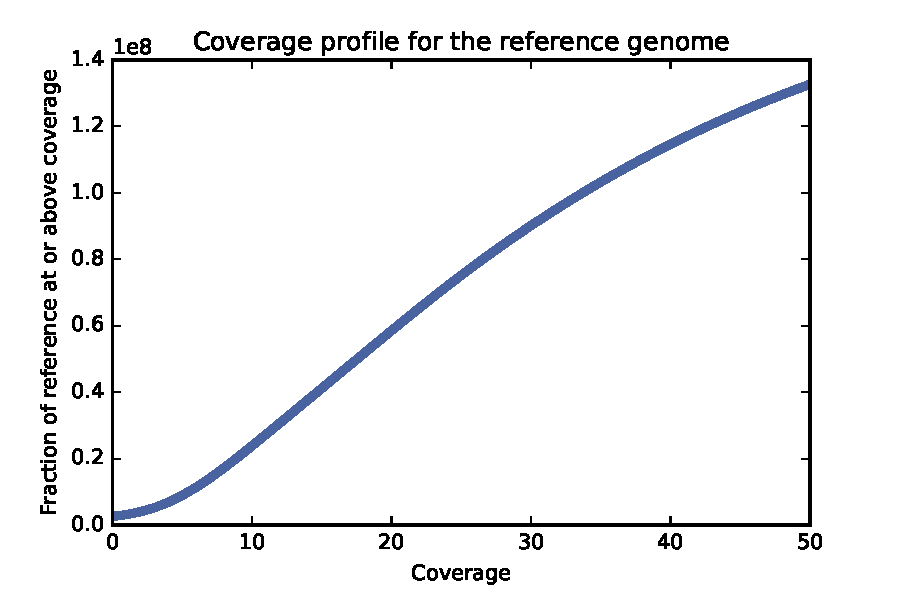
\includegraphics[width=0.45\textwidth]{CoverageProfile.pdf}  
\caption{\label{fig:coverage-profile} Cumulative coverage profile for the reference metagenome, based on read mapping. }
\end{figure}

%\begin{figure}[!h]
%\centering
%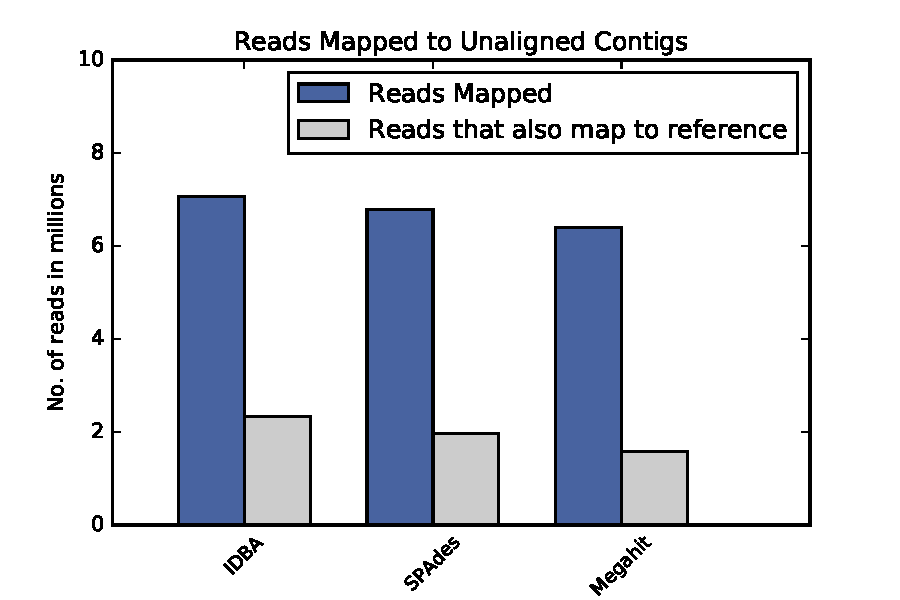
\includegraphics[width=0.45\textwidth]{UnalignmentHistogram.pdf} %to be chamged to qc.coverage-profile
%\caption{Mapping unaligned reads to reference genome using identity 99\%, and Ambiguous Approach CTB This can't be right :)}
%\label{fig:unaligned-reads}
%\end{figure}

% \begin{figure}[!ht]
% \centering
% 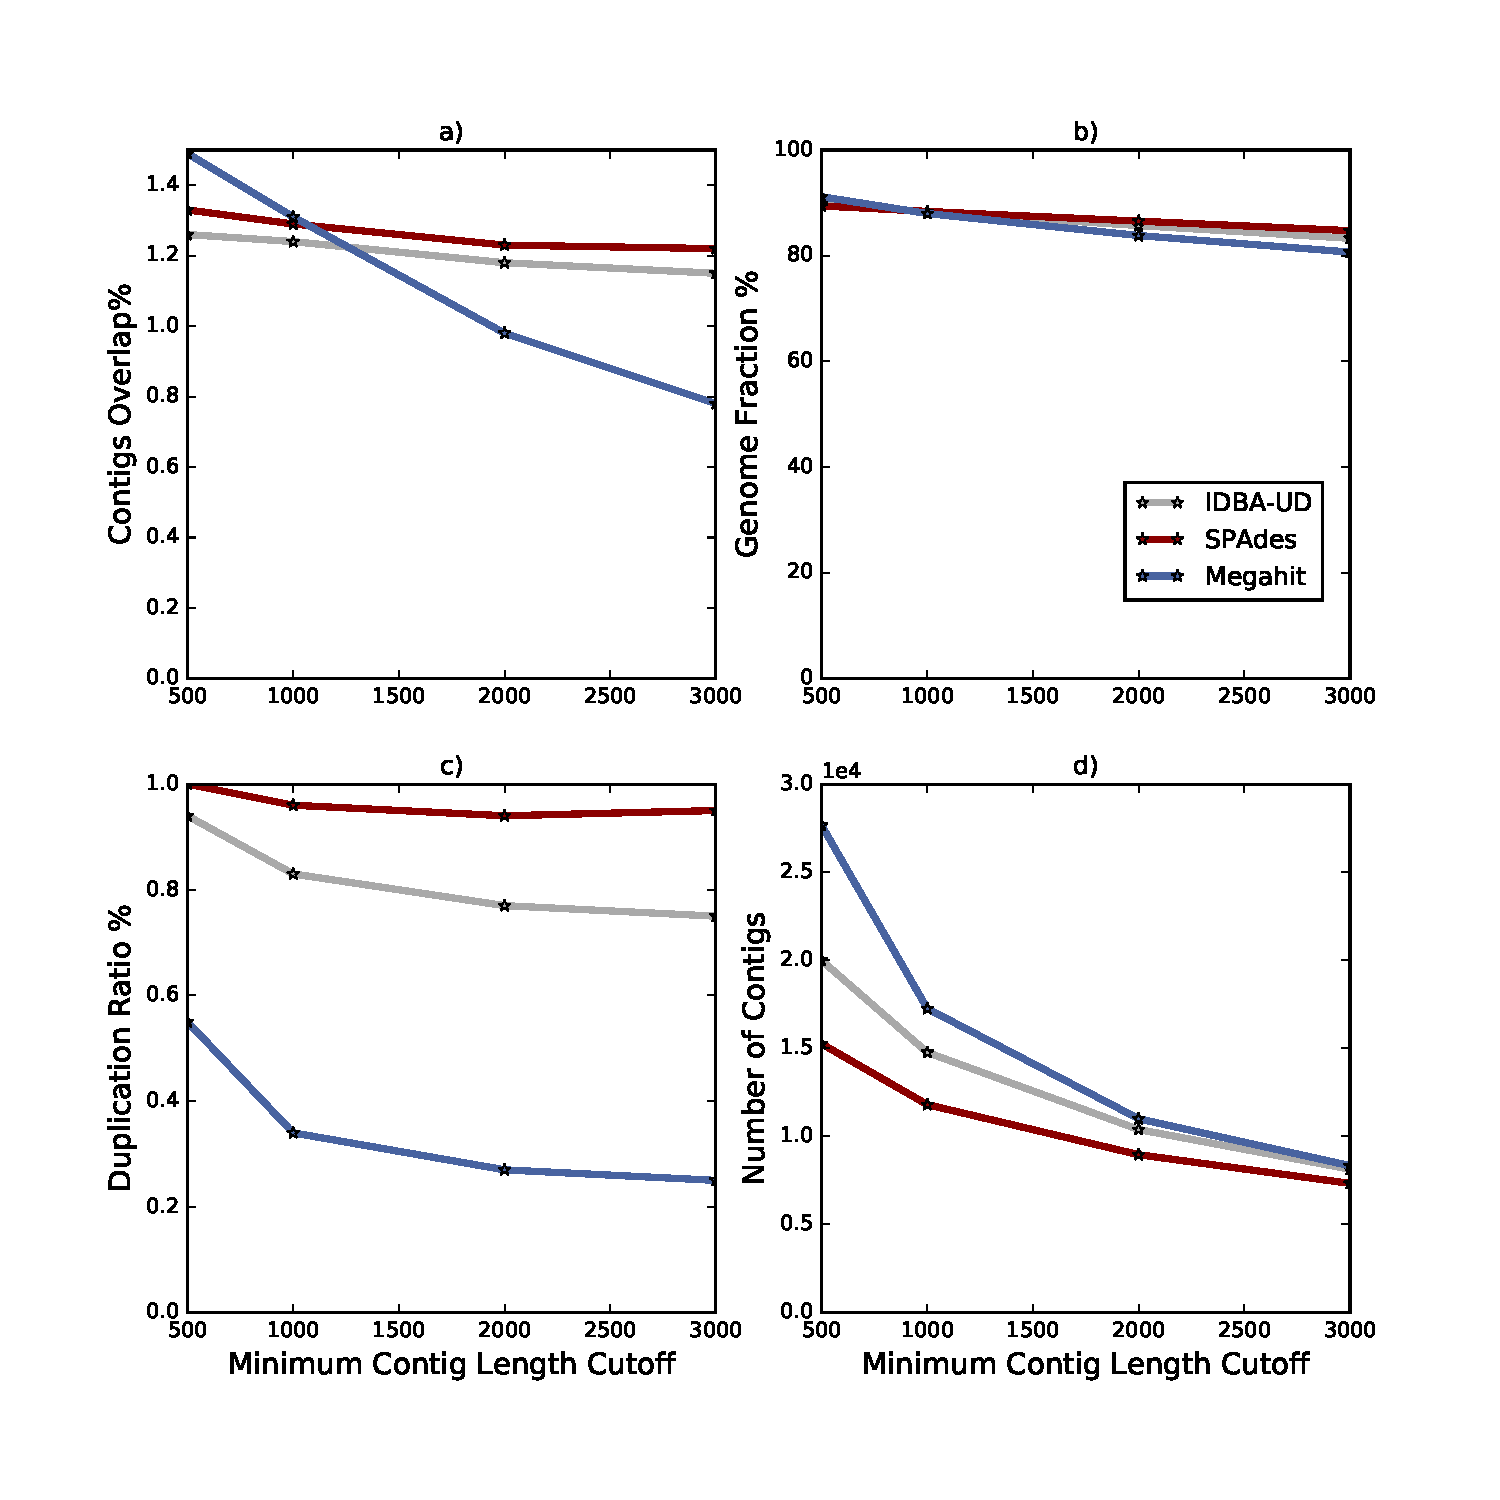
\includegraphics[width=9.5cm,height=9.5cm]{min-contig-analysis.pdf}  
% \caption{\label{fig:min-contig-analysis} Genome fraction, duplication ratio, Contigs overlap ratio, and number of contigs using different minimum contig length,  identity 99\%, and Ambiguous Approach}
% \end{figure}

% \begin{figure}[!h]
% \centering
% 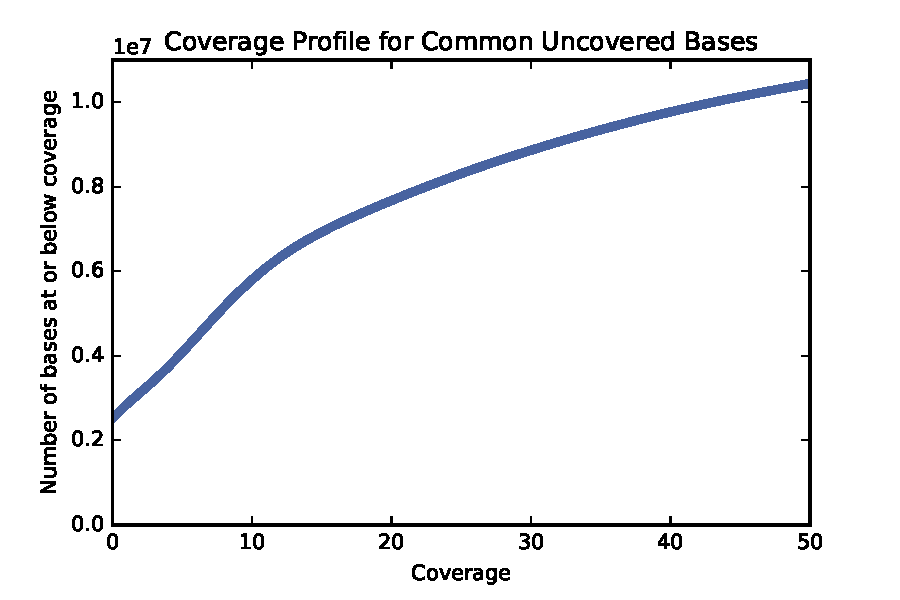
\includegraphics[width=0.4\textwidth]{CommonUncoveredCoverageProfile.pdf} 
% \caption{Cumulative read coverage for bases in the reference metagenome missing from all three assemblies.}
% \label{fig:CommonUncovered}
% \end{figure}



% \begin{figure}[!h]
% \centering
% \includegraphics[width=0.4\textwidth]{MapQuality.png}  
% \caption{\label{fig:mapquality} Mapping Quality for Quality Filtered Reads to the Reference Genome}
% \end{figure}

% \begin{figure}[!h]
% \centering
% \includegraphics[height=2.6cm,width=0.4\textwidth]{basequality.png}  
% \caption{\label{fig:basequality} Mean Base Quality}
% \end{figure}

% \begin{figure}[!h]
% \centering
% \includegraphics[height=2.6cm, width=0.4\textwidth]{errorprofile30.png}  
% \caption{\label{fig:errorprofile30}Error Profiles for MAPQ >=30}
% \end{figure}

% \begin{figure}[!h]
% \centering
% \includegraphics[height=2.6cm, width=0.4\textwidth]{nucleotidecomposition.png}  
% \caption{\label{fig:nucleotidecomposition.png}Nucleotide Composition for MAPQ >=30}
% \end{figure}
% \subsection*{Mathematics}

 
% \subsection*{Mathematics}

\subsection*{Datasets}
%Numbers in this section are up to date 22 december 2016

We used a diverse mock community data set constructed by pooling DNA
from 64 species of bacteria and archaea and sequencing them with
Illumina HiSeq.  The raw data set consisted of 109,629,496 reads from
Illumina HiSeq 101 bp paired-end sequencing (2x101) with an untrimmed
total length of 11.07 Gbp and an estimated fragment size of 380 bp
\cite{podar}.
 
The original reads are available through the NCBI Sequence Read
Archive at Accession SRX200676.
We received the 64 reference genomes from the original authors. They
consist of 205.6 Mbp of assembled genomes in 64 contigs, and are
available for download at
https://dx.doi.org/10.6084/m9.figshare.1506873.v2

\section*{Methods}
The analysis code and run scripts for this paper are available at:
https://github.com/dib-lab/2015-metagenome-assembly/. The scripts and
overall pipeline were examined by the first and senior authors for
correctness.  In addition, the bespoke reference-based analysis
scripts were tested by running them on a single-colony E. coli MG1655
data set which had a high quality reference genome (cite Chitsaz,
2011).

\subsection*{Quality Filtering} 

We removed adapters with Trimmomatic v0.30 in paired-end mode with the
Truseq adapters \cite{trimmomatic}, using light quality score trimming
as recommended in @cite MacManes 2014.

%We next used the fastq\_quality\_filter from the FASTX-Toolkit v0.0.13.2  \cite{FXtoolkit} to remove sequences using the parameters  {\tt{-Q33   -q 30 --p 50}} , which keeps all sequences with  50\%  or more bases with quality score greater than or equal to 30.

\subsection*{Reference Coverage Profile}

To evaluate how much of the reference metagenome was contained in the read
data, we used {\tt bwa aln} to map reads to the reference genome.  We then
calculated how many reference bases were covered by how many mapped
reads (custom script {\tt coverage-profile.py}).

\subsection*{Assemblers}
We assembled the quality-filtered reads using three different assemblers: IDBA-UD
\cite{idba}, SPAdes \cite{spades}, and MEGAHIT \cite{megahit}.  For
IDBA-UD v1.1.1 \cite{idba}, we used {\tt {--pre\_correction}} to
perform pre-correction before assembly and -r for the pe files.

For SPAdes v3.9.0 \cite{spades}, we used { \tt {--meta --pe1-12
    --pe1-s}} where {\tt{--meta}} is recommended when working with
metagenomic data sets, {\tt{--pe1-12}} specifies the interlaced reads
for the first paired-end library, and {\tt{--pe1-s}} provides the
orphan reads remaining from quality trimming.

%@SAM this is what we used?  
For MEGAHIT \cite{megahit}, we used -l 101 {\tt{-m 3e9
    --cpu-only}} where {\tt -l} is for maximum read length, {\tt -m} is
for max memory in bytes to be used in constructing the graph, and {\tt
  {--cpu-only}} to use only the CPU and not the GPU. We also used {\tt
  {--presets meta-large}} for large and complex metagenomes, and {\tt
  {--12} } and {\tt{-r}} are parameters that specify the
interleaved-paired-end and single-end files respectively.

All three assemblies were executed on the same high-memory buy-in node
on the Michigan State University High Performance Compute Cluster, and
we recorded RAM and CPU time of each assembly job using the {\tt
  qstat} utility at the end of each run.

Unless otherwise mentioned, we eliminated all contigs less than 500 bp
from each assembly prior to further analysis.

\subsection*{Mapping}

We aligned all quality-filtered reads to the reference metagenome with
bwa aln (v0.7.7.r441) \cite{bwa}. We aligned paired-end and orphaned
reads separately using bwa aln samse. We then used samtools (v0.1.19)
\cite{sam-stools} to convert SAM files to BAM files for both
paired-end and orphaned reads. To count the unaligned reads, we
included only those records with the ``4'' flag in the SAM files
\cite{sam-stools}.
 

To extract the reads that contribute to unaligned contigs, we mapped
the quality filtered reads to the unaligned contigs using bwa aln
(v0.7.7.r441) \cite{bwa}.  Then we used samtools to retrieve the reads
that mapped to the unaligned contigs.


%We found chimeric alignments (alignments that split reads in two or more) with the bwa mem aligner using the default parameters (v0.7.7.r441). 

%To count the chimeric alignments, we count the secondary alignments (records with the ``SA" flag) in the SAM file \cite{samtools}. 

%We used SamStats \cite{samstats} to analyze the quality of mapping and errors. 

\subsection*{k-mer Presence}
In order to examine k-mer presence for a k-mer size of 20, we built a
k-mer counting table from the given quality filtered reads using
{\tt{load-into-counting.py}} from khmer (@cite khmer). Then we
calculate abundance distribution of the k-mers in the quality filtered
reads using the pre-made k-mer counting table using
{\tt{abundance-dist.py}}. We followed the same approach to examine
k-mer presence in assemblies.

\subsection*{Assembly analysis using Nucmer}

We used the Nucmer tool from MUMmer3.23 \cite{mummer3.0} to align
assemblies to the reference genome with options {\tt \--coords} {\tt
  -p}. Then we parsed the generated ``.coords'' file using a custom
script {\tt{analyze\_assembly.py}} to calculate several analysis
metrics across all the assemblies at two alignment identities, 95\% and 99\%.

\subsection*{Reference-based analysis of the assemblies}
We processed the alignments in three different ways: ambiguous,
best-hit, and no-misassemblies.

% In the ambiguous approach, we keep all alignments, including alignments where multiple contigs align to the same region in the reference, and multiple parts of the same contig align to the same reference region. Alignments to different parts of the reference are kept too. 

% In the best-hit approach, when different parts of one contig align to the reference, we only take into account the highest-scoring alignment and discard the other alignments from that contig.

% In the no-misassemblies approach, we count only contigs that align uniquely and completely to the reference. If the contig aligns partially, or different parts of the contig align to different regions in the reference, we discard all of the alignments.


In the ambiguous approach, we took into account all the alignments of
a contig to the reference.

In the best-hit approach, among all alignments of a contig, we took
into consideration only the alignment with the best score.

In the no-misassemblies approach, we only counted contigs that have
precisely one alignment to the reference.

In all approaches, we flag a base in the reference genome as
``covered'' if it is contained in a kept alignment.  We define the
duplication ratio as the percentages of bases in the reference covered
by two or more kept alignments. We define misassemblies as
those contigs that are divided into different parts when mapped to the
reference.  The number of misassembled contigs is equal to the number
of aligned contigs (both totally and partially) in the ambiguous
approach, minus the number of aligned contigs in the no-misassemblies
approach.

%We define the contig overlap ratio as the number of bases
%aligned to the reference that exist in more than one contig.  We
%define the contig overlap ratio as the number of bases aligned to the
%reference that exist in more than one kept alignment.

All approaches have a non-zero duplication ratio within the reference
because we do not explicitly discard contigs that map to the same
location in the reference.


\subsection*{Gene annotations using Prokka}
We used prokka \cite{prokka} to annotate the reference genome using
{\tt{--outdir mprokka --prefix testasm --metagenome}}. Then we parsed
the testasm.tbl output file to get the coordinates of CDS genes. We then
searched the alignments for how many genes were contained in those
alignments.
% @CTB what script?

\section*{Results}

\subsection*{The raw data is high quality}

We trimmed sequences as described in Methods. We retained 7.1 Gbp in
108,422,358 paired-end sequences, and 36 Mbp in 520,403 orphaned
reads.  This quality trimmed ("QC") data set was used as the basis for
all further analyses.

%\subsection*{Mapping Quality and Error Profiles}

%%Might need to be merged with previous section  @CTB
%We used SAMStat \cite{samstat} to analyze the mapping quality and error profiles of quality filtered reads mapped to the reference genome. Figure \ref{fig:mapquality} shows number of alignments in various mapping quality (MAPQ) intervals and number of unmapped sequences. The percentage and number of alignments in each category is given in brackets. 
%Figure \ref{fig:basequality} shows mean base quality of reads with low and high mapping quality. %Figure \ref{fig:errorprofile30} shows the error profile for MAPQ $\geq 30$ and Figure \ref{fig:nucleotidecomposition.png} shows the nucleotide compositions. We also found 309,414 chimeric reads. 

\subsection*{98\% or more of the reference is present in the read data set}

We next evaluated the fraction of the reference genome covered by at least
one read (see Methods for details). Quality filtered reads cover
203,058,414.0 (98.76\%) bases of the reference metagenome (205,603,715
bp total size).  Figure \ref{fig:coverage-profile} shows the
cumulative coverage profile of the reference metagenome, and the
percentage of bases with that coverage. Most of the reference
metagenome was covered at least minimally; only 3.33\% of the
reference metagenome had mapping coverage \textless 5, and 1.24\% of
the bases in the reference were not covered by any reads in the QC data
set.

In order to evaluate reconstructability with De Bruijn graph
assemblers, we next examined k-mer presence for a k-mer size of 20. Of
the 174m 20-mers in the reference metagenome, 98.7\% were present in the
QC reads and 95.5\% of them occurred with abundance 5 or greater in
the QC reads.

%Data source note: the 95.5 is from
% SRR606249.qc.dist (1-0.045)*100 , the 98.7 is from the same file but
% (1-0.013) *100

\subsection*{MEGAHIT is the fastest and lowest-memory assembler evaluated}
%Numbers in this section are up to date 22 december 2016

We ran three commonly used metagenome assemblers on the QC data set:
IDBA-UD, SPAdes, and Megahit. We recorded the time and memory usage of
each (Table \ref{table:time-memory}).  MEGAHIT outperformed both
SPAdes and IDBA-UD considerably, producing an assembly in one hour --
approximately 17 times faster than IDBA and 42 times faster than
SPAdes.  MEGAHIT used only 34.4 GB of RAM -- 1/5 to 1/11th
the memory used by IDBA and SPAdes, respectively.

\subsection*{The assemblies contain most of the raw data}
%Numbers in this section are up to date 22 december 2016

The assemblies represent the majority of the k-mers in the reads (99.7\% of
the unique k-mers in the reads are present in the assembly) and
the majority of the high abundance 20-mers (93.7\% of the abundance
\textgreater 5 20-mers in the reads), suggesting that the assemblies
represent the underlying content of the reads very well.

% %the 93.7 is from qc500.dist (1-0.027)*100.
% the 99.7% is from  (1-0.003)*100

% @CTB fixme section

\subsection*{Much of the reference is covered by the assemblies}
%Numbers in this section are up to date 22 december 2016

We next evaluated the extent to which the assembled contigs recovered the
``known/true'' metagenome sequence by aligning each assembly to the
reference (Table ~\ref{table:coverage-analysis}).  All three
assemblers generate contigs that cover more than 89\% of the reference
metagenome at high identity (99\%) with little duplication
(0.55 -1.0\%) (see "Ambiguous approach" in
Table~\ref{table:coverage-analysis}).  If we relax the identity
threshold to 95\%, then the assembled contigs cover more than 94\% of
the reference metagenome.

% @CTB note for discussion: so here the assemblies approximate the
% best possible, as measured by high-coverage bases/k-mers.

When we use only the highest-scoring alignment at 99\% identity, we
find that the reference coverage drops to 57-68\%, depending on the
assembler ("Best hit approach",
Table~\ref{table:coverage-analysis}). The reference coverage from
highest-scoring alignments does not substantially increase when the
identity threshold is relaxed to 95\%.

At 99\% identity with the ambiguous approach, approximately 6.23\% of
the reference is covered by no contig from any of the three
assemblies; we discuss this in more detail below.
%common uncovered / no.of bases in the reference *100
% @CTB we need to extend methods to contain mention of common uncovered.
% Probably belongs in the ``Analyzing Assembly'' section.

\subsection*{The generated contigs are broadly accurate} 
%Numbers in this section are up to date 22 december 2016

When counting only the best alignment per contig at a 99\%
identity threshold, more than 72\% of contigs align to the reference
completely, i.e. across the whole length of the contig (Table~\ref{table:contigs-analysis}, ``Best hit'', Totally Aligned Contigs \%).  If we allow
multiple alignments per contig, then more than 80\% of contigs align
completely (although not contiguously) to the reference (Table~\ref{table:contigs-analysis}, ``Ambiguous'', Totally Aligned Contigs \%).
Approximately 4 - 9\% of the contigs align only partially, and the
remaining 8 - 10\% of contigs do not align at all to the reference
(discussed in detail below).

\subsection*{All three assemblers perform equally well in reference base recovery}
%Updated on 27 December  

%we have 6.23% of the reference is commonly uncovered. We have 0.64% of bases covered by IDBA only, 0.74% of bases covered by SPAdes only, and 1.92% of bases covered by Megahit only.  Each uniquely fail to recover about 1\% (1.22-1.79\%) of the reference. XX is roughly.

90.47\% of the reference metagenome is recovered in at least one
contig by all three assemblers (``common covered'') with relatively
little duplication, under 99\% identity/ambiguous matching: 6.23\% of
the reference is missed by all three assemblers, 0.64\% is recovered
by IDBA alone, 0.74\% is recovered by SPAdes only, and 1.92\% is
recovered by MEGAHIT only.

% @CTB sherine, does this make sense? I just summed the numbers...
% I can't think straight about it.

Of the uncovered bases in common between the assemblers, 19.66\% have
zero mapping coverage, while 29.20\% have mapping coverage \textless
5.
%(@CTB what can we say about the rest?!)

% @CTB update with number of bases; check numbers in source files.
% @CTB what can we say about the rest? anything?
%(Using awk '$1 <5 {sum +=
%$2} END {print sum}' common-uncovered-coverage.out)/no. common
%  uncovered bases from analyze_assembly.py output *100
% @CTB make sure to discuss this!

IDBA, SPAdes, and MEGAHIT each uniquely fail to recover about
1\% of the reference.

\subsection*{Large portions of several reference genomes are not assembled by any assembler}
%Numbers in this section are up to date 21 december 2016

A number of the genomes in the reference metagenome had many missing
bases in the assemblies (Table ~\ref{table:genomes_uncovered}). In
three extreme cases, {\em Shewanella baltica OS223}, {\em Fusobacterium
nucleatum}, and {\em Desulfovibrio vulgaris} contribute 18.25\%, 16.95\%, and 12.85\%
of the total common uncovered bases respectively.

%these numbers are after sorting file QC.AMBIGUOUS.99.uncovered using
%[sort -n -k2 -r  QC.AMBIGUOUS.99.uncovered>QC.AMBIGUOUS.99.uncovered.sorted ] and the percentage is computed w.r.t no. of common uncovered bases

% @CTB: we need to add in percentages of the genome, I think, as well.

\subsection*{Most genes within the reference metagenome are contained within contigs}
%Numbers in this section are up to date 21 december 2016

The reference genome has 188,880 CDS with 91,806 annotated as genes,
based on a Prokka annotation (see Methods).
Using the ``ambiguous'' alignment approach and 99\% identity, the
IDBA-UD assembly contained 82,791 (95.20\%) of the reference genes,
while SPAdes contained 83,475 (94.44\%), and
MEGAHIT contained 80,256 (94.59\%) of the reference genes.

%These numbers are from prokka-analysis.out.
%also see prokka.out and mprokka/testasm.tbl
% @CTB are these in a table anywhere?

% second tier todo - @CTB what about taking the nucleotide sequences
% output by prokka and see if they match in the assembly?

\subsection*{Many assembled contigs do not align to the reference metagenome}

Depending on assembler, between 8.04\% and 10.87\% of the assembled
contigs (XX-YY bases total) do not align anywhere in the reference
metagenome.  We extracted these contigs and analyzed their content and
read mapping separately.

Between 5.9and 6.5\% of the QC reads mapped to the unalignable
contigs, depending on assembler (@CTB put in table).  In each case,
between 67\% and 75\% the reads that mapped to these unalignable
contigs did not map anywhere in the reference (put in table); about 5m
QC reads total map only to the unaligned contigs and nowhere in the
reference.

%6.49\% of reads mapped to the unaligned contigs of IDBA. Only 33.01\%
%of those reads mapped to the reference. (2.14\% of all the reads).
%6.23\% of reads mapped to the unaligned contigs of SPAdes. Only
%28.97\% of those reads mapped to the reference. (1.80\% of all the
%reads).  5.87\% of reads mapped to the unaligned contigs of
%Megahit. Only 24.80\% of those reads mapped to the reference. (1.45\%
%of all the reads)
%The above numbers are coming from
%iqc.AM99.aligned.reads and iqc.AM99-mapped-reads for IDBA,
%sqc.AM99.aligned.reads and sqc.AM99-mapped-reads for SPADES, and
%mqc.AM99.aligned.reads and mqc.AM99-mapped-reads for megahit.
For
each assembly, approximately 5m quality-filtered reads map only to the
unaligned contigs (and nowhere in the reference).
%Numbers from subtracting numbers in those files:
%(iqc.AM99.aligned.reads - iqc.AM99-mapped-reads) for IDBA
%(sqc.AM99.aligned.reads - sqc.AM99-mapped-reads) for SPAdes 
%(mqc.AM99.aligned.reads - mqc.AM99-mapped-reads) for megahit

% For IDBA QC, the reads that aligned to the unaligned contigs but not
% to the reference has coverage bases 27.21\% \textless 5 in the
%unaligned contigs. 75.72\% has coverage \textgreater 0.

% For SPAdes QC, the reads that aligned to the unaligned contigs but not
% to the reference has coverage bases (3,109,539) 24.04\% \textless 5 in
% the unaligned contigs. 79.10\% has coverage \textgreater 0.

% For Megahit QC, the reads that aligned to the unaligned contigs but
% not to the reference has coverage bases (2,578,896) 20.18\% \textless
% 5 in the unaligned contigs. 83.08\% has coverage \textgreater 0.

%The above numbers are coming from iqc.unmapped.out, sqc.unmapped.out, and mqc.unmapped.out

We used sourmash (cite) to search the unalignable contigs against all
52,000 microbial genomes currently available from NCBI and found nine
genomes with significant estimated overlap with the unalignable contigs
(10\% or more estimated overlap - @CTB put in Methods).  We then
aligned the unalignable contigs against these nine genomes, and found
that between 16\% and 28\% of the previously unaligned contigs matched
to the new genomes at 99\% identity.

% \subsection*{Pending text: To add or not}
% Figure \ref{fig:min-contig-analysis} shows the number of contigs using
% different minimum contigs cutoff.  The figure shows that Megahit
% \cite{megahit} has more fragmented contigs in the assembly. The small
% contigs size leads to best alignment; Megahit has the highest number
% of uniquely covered bases, highest genome coverage, and lowest
% unalignment.

\section*{Discussion}
\subsection*{Assembly recovers basic content well}

%Updated on 26-28 December 
The majority of the reference metagenome is recovered by all three
assemblers: 89\% or more of the reference metagenome is contained
within each assembler’s output at 99\% identity, and 94\% can be
recovered if we relax the identity threshold to 95\%.  This is close
to the measured maximum reconstructability based on read mapping and
k-mer presence: 98.76\% of the reference is covered by at least one
read, and 98.7\% of the genome is present in k-mers of size 20.
%98.76
%and 98.7 are from SRR606249.qc.coverage and SRR606249.qc.dist
%respectively

The contigs generated align well to the reference metagenome: with all assemblers, 80\% (or
more) of contigs align to the reference metagenome across the whole
length of the contig, and another 4\% (or more) of the contigs are
entirely contained within the reference metagenome, although they do
not align to only one location in the reference.

% @CTB add note: This could be caused
% by misassembly (a computational error) or by rearrangements in the
% source DNA (in which case the reference is incorrect).
 
%(Talk about gene content of assemblies here.)
%Updated on 27 December 
More than 6.23\% of the reference metagenome is missing from all of
the assemblies when 99\% similarity is required, and large portions of
the missing sequence are from a few genomes -- in some cases, close to
a fifth of the source genome is missing from the assemblies.
About a third of the missing reference (29.2\%) is low coverage based on
read mapping, but the remainder has read coverage greater than 5.
(Chase this down descriptively.)
% @CTB chase this down.

%6.23 is the (12,807,937 bases)/205603715 *100: all coming from assemblies.stats.QC.AMBIGUOUS.99 

%932,873 out of these missing bases are GC bases.

%The read coverage
%of the unassembled regions of the source genome is low to nonexistent
%, while other portions of the source genomes are well represented
%within the reads; these regions were simply not sequenced, either
%because they were missing from the input DNA or because they challenge
%the sequencer. %However, some unassembled regions have good coverage:
%we have only 29.2% with coverage <5 in the common uncovered.

@CTB here mention gene recovery/prokka etc is good.


\subsection*{Assembly produces contiguous sequence not in the reference metagenome}
%@CTB: I don't know what XX in this section refering to. 
% XX was >5 is comming from iqc.unmapped.out, sqc.unmapped.out, and mqc.unmapped.out where ~75% of the reads mapped to the aligned contigs and not to the reference has coverage of one at least in the contigs, but the text refers to ccontigs coverage? so something here doesn't add up;

In addition to recovering most of the content of the reference
metagenome, all three assemblers generate many contigs (approximately
10\% of the total) that do not map to anything in the reference.
While some could be misassemblies, many of the reads that map to these
contigs do not map anywhere in the reference, while many of the
contigs have coverage >XX, suggesting that they are present within the
source DNA at an abundance that is similar to many of the genomes in
the mock community.

(@CTB identify etc.)

%This part I left as it is.

Whatever their true identity, these contigs are not present in the
reference metagenome. Because this is a mock metagenome for which
isolates were grown and individually extracted prior to being combined
for sequencing, we believe that these extra genomic contigs must come
from one or more contaminants.  We cannot rule out contamination from
kits, but because large amounts of DNA were used to create the mock
community, it seems unlikely that these are due to trace contaminants
created by PCR (as can happen in amplicon studies); they are most
likely from contaminants grown together with the isolates.

\subsection*{Different assemblers differ in content recovery, but not by much}
%Updated on 24 December :@CTB still need the XX from: we have 6.23% of the reference is commonly uncovered. We have 0.64% of bases covered by IDBA only, 0.74% of bases covered by SPAdes only, and 1.92% of bases covered by Megahit only.  Each uniquely fail to recover about 1\% (1.22-1.79\%) of the reference.

The three assemblers differ very little in recovery of basic content,
as judged by reference metagenome alignments: at 99\% identity, XX\%
is recovered in common, with 0.64 to 1.92\% specific to each assembler
(and a total of XX\% being recovered by one or two, but not all three,
of the assemblers). None of the assemblers include all of the sequence
produced by the others, suggesting that assembler-specific heuristics
are responsible for the variation.

. %, and the extra sensitivity offered by
%MEGAHIT comes with a higher level of duplication.
%I commented the previous sentence as Megahit is not the lowest in duplication 

\subsection*{Genome assembly metrics are misleading}

\begin{itemize}
\item content recovery is of first importance IMO
\item contig n50/ng50 comparison?
\item longer contigs lead to more misassemblies; suggest avoiding until long reads work well for metagenomes
\item but long reads don't yet work well for metagenomes due to diversity
\item fosmid type approaches maybe? moleculo etc.
\end{itemize}

\subsection*{Recommendation: try MEGAHIT first}

We do not see a significant advantage to one assembler over another in
terms of recovering the known reference, and we speculate that there
is little advantage to combining assemblies from multiple assemblers,
since very little extra content will be recovered.

While the other assemblers produce longer contigs, we are concerned by
misassembly rates, which affect longer contigs disproportionately.
Moreover, misassemblies are hard to detect without a reference. 
(Talk
more about misassemblies.)

For these reasons, our recommendation is to use MEGAHIT with
short-read data: it is significantly faster and lower memory than
SPAdes and IDBA-UD, recovers essentially the same content, and -- for
short read data sets -- does not offer significant disadvantages in
terms of contig length.

(Here note that megahit does not allow long reads, unlike SPAdes and maybe
IDBA. @CTB verify this.)

\section*{Conclusions}

Assembly works well. There is no big difference between assemblers'
performance in terms of assembly quality. In terms of cost, Megahit is
much faster and utilizes less memory.

\begin{itemize}
\item If you have short-read sequencing only, use MEGAHIT.
\item MEGAHIT can be useful for exploratory analysis of content as well.
\item Metagenome assembly is good at recovering content of well covered
  regions.  It is less good at long-range contiguity. It is better than
  reference based analysis at recovering content.
\item Resequence mock community genomes, as in evolutionary studies.
\end{itemize}

% @CTB mention long reads, microdiversity (banfield study).
% consequences for genome binning etc.

% do we make comments about tradeoff between single contig analysis,
% quast analysis, etc?
% better misassembly analysis?
% do we want to bring in REAPR or whatnot? does it work OOB for metagenomes?

\subsection*{Author contributions}
In order to give appropriate credit to each author of an article, the
individual contributions of each author to the manuscript should be
detailed in this section. We recommend using author initials and then
stating briefly how they contributed.

\subsection*{Competing interests}
No competing interest to our knowledge.

\subsection*{Grant information}
This work is funded by Moore and NIH.

\subsection*{Acknowledgments}
Michael R. Crusoe

{\small\bibliographystyle{unsrtnat} \bibliography{references}}

\bigskip
% References can be listed in any standard referencing style that uses a numbering system
% (i.e. not Harvard referencing style), and should be consistent between references within
% a given article.

% Reference management systems such as Zotero provide options for exporting bibliographies as Bib\TeX{} files. Bib\TeX{} is a bibliographic tool that is used with \LaTeX{} to help organize the user's references and create a bibliography. This template contains an example of such a file, \texttt{references.bib}, which can be replaced with your own. Use the \verb|\cite| command  to create in-text citations, like this .


% See this guide for more information on BibTeX:
% http://libguides.mit.edu/content.php?pid=55482&sid=406343

% For more author guidance please see:
% http://f1000research.com/author-guidelines


% When all authors are happy with the paper, use the 
% ‘Submit to F1000Research' button from the menu above
% to submit directly to the open life science journal F1000Research.

% Please note that this template results in a draft pre-submission PDF document.
% Articles will be professionally typeset when accepted for publication.

% We hope you find the F1000Research Overleaf template useful,
% please let us know if you have any feedback using the help menu above.


\end{document}

